% !TEX root =  ../master.tex
\chapter{Konzeption}\label{cha:konzeption}
Bevor mit der Implementierung gestartet werden kann wird ein Konzept erstellt, welches dann als Leitfaden für die Implementierung dienen soll.
Ziel ist ein konkreter Entwurf, welcher die technischen und grundlegenden Funktionalitäten beschreibt.
Dadurch soll verhindert werden, dass die aufwendige Implementierung fehlschlägt oder mehrfach Änderungen durchgeführt werden müssen, wodurch der Implementierungsaufwand vergrößert würde.


















\section{Konzeption der Anwendungsarchitektur}
Die Grundlage jeder Anwendung ist der Aufbau und die Struktur der Infrastruktur, auf welcher die Anwendung später ausgeführt werden soll.
Aus diesem Grund wird diese als Erstes betrachtet.

\subsection{Traditionelle Architektur}

Webanwendungen werden üblicherweise in einem Client-Server-Modell entwickelt. Im Konkreten kann hier von einer Thin-Client Architektur gesprochen werden, da jegliche Anwendungsdatenverarbeitung Server-seitig durchgeführt wird \autocite{definitionOfThinClient}.
Der Client übernimmt dabei sämtliche Funktionalitäten, die das Nutzerinterface betreffen. Über diese Aufteilung von Verantwortlichkeiten können Wartung und Sicherheit durch die zentrale serverseitige Verwaltung in einem Rechenzentrum einfacher gesichert werden. Falls der Client selbst Daten verarbeiten und speichern würde, könnte dies zu inkonsistenten Daten und Sicherheitslücken führen, da unterschiedliche Datenbestände zwischen Client und Server entstehen könnten. 
Visualisierung und die Interaktion mit dem Nutzer fallen hierbei in die Aspekte des Nutzerinterfaces, worüber diesem die Interaktion mit den zentralen Datenbeständen ermöglicht wird. Dabei wird jedoch keine Anwendungslogik ausgeführt \autocite{thinClientArchitectureOverview}. Es ist allerdings wichtig zu betonen, dass diese Nutzerschnittstelle essentiell für den Erfolg der Anwendung ist. Eine maximale User Experience \autocite{definitionUserExperience} zu bieten ist ein kritischer Faktor für die Qualität der Nutzerschnittstelle \autocite{thinClientArchitectureOverview}.\\
Entsprechend wird die gesamte Geschäftslogik, Datenhaltung und der Datenaustausch von einem zentralen Server verwaltet. 
In \autoref{fig:clientServerAufbau} ist eine solche Architektur vereinfacht dargestellt, wobei zwischen dem Anwendungs- und dem Datenbankserver unterschieden ist. Der Anwendungsserver beinhaltet hierbei sämtliche Geschäftslogik- und Datenaustauschzuständigkeiten. Der Datenbankserver ist hingegen ausschließlich für die persistente Datenhaltung zuständig.

\begin{figure}[h]
    \centering
    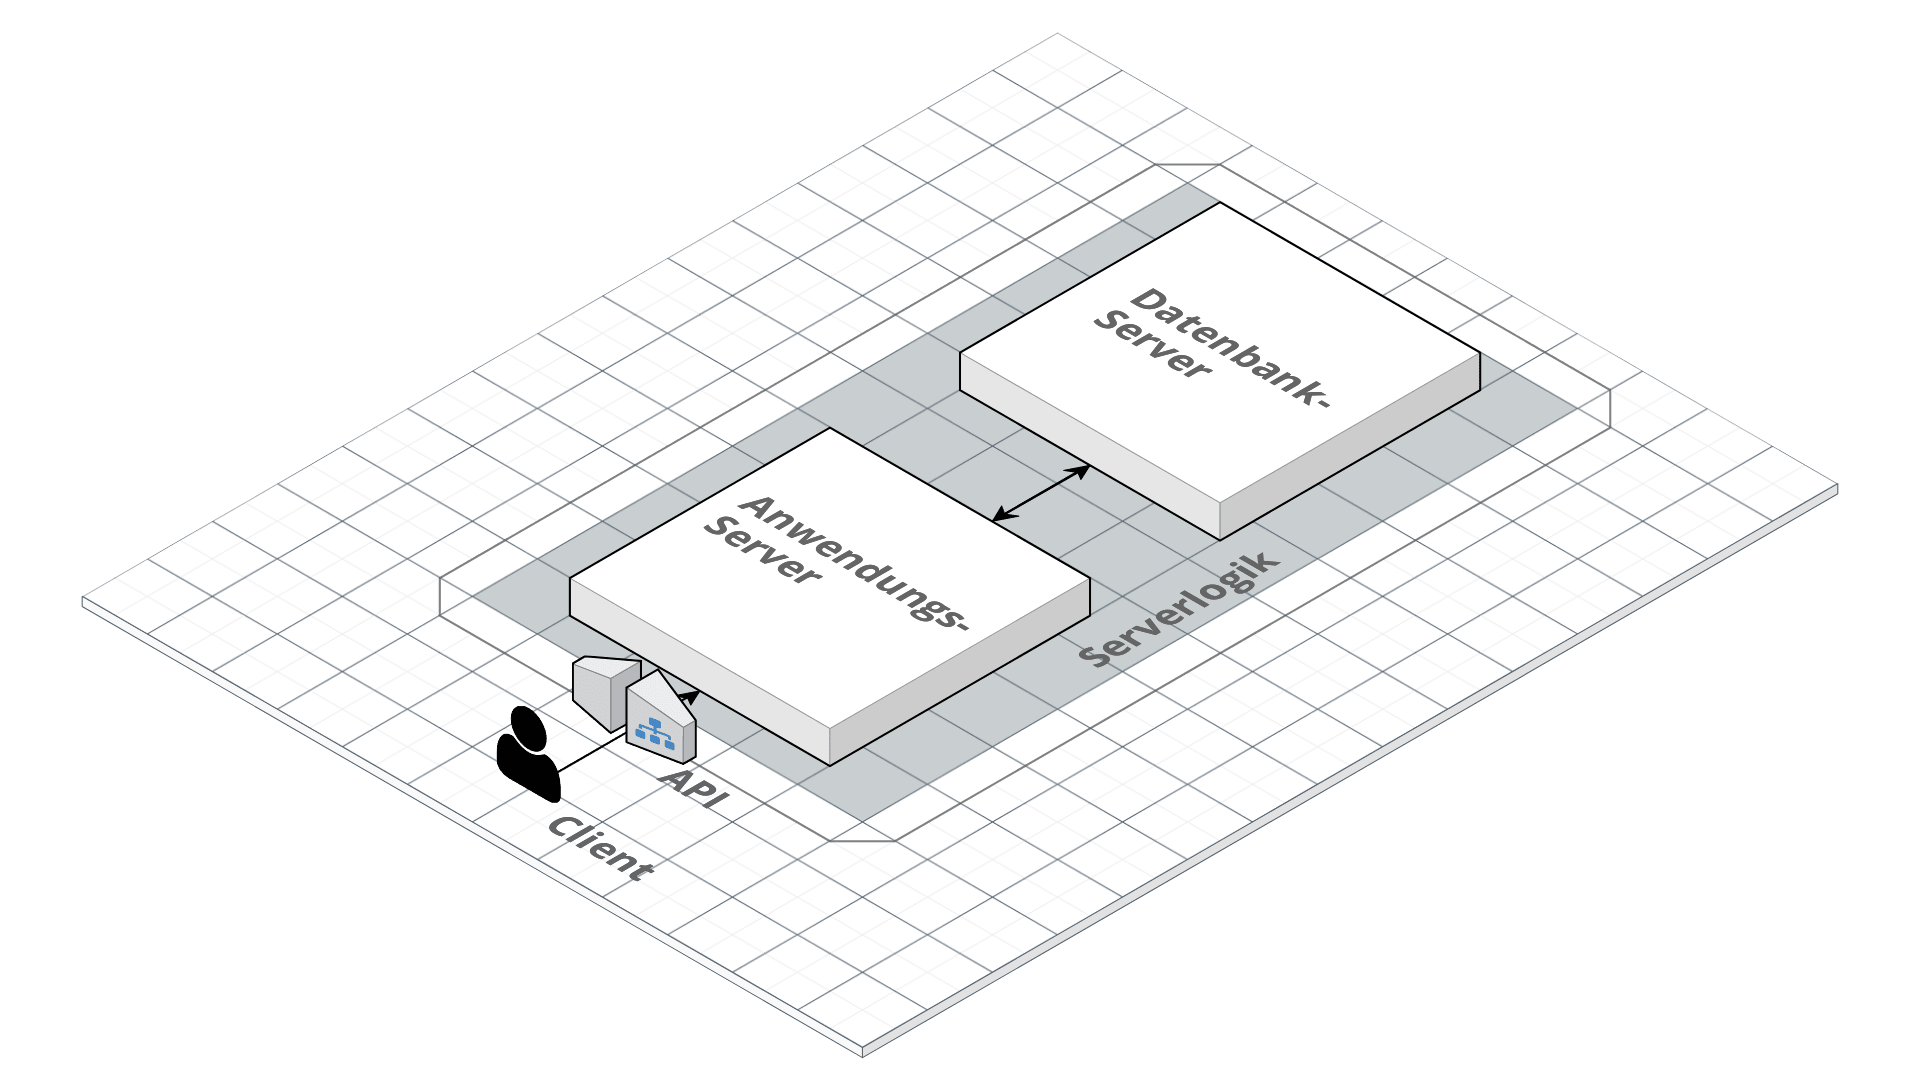
\includegraphics[width=.9\textwidth]{img/ClientServer.png}
    \caption{Vereinfachter Client-Server-Aufbau}
    \label{fig:clientServerAufbau}
\end{figure}

Praktisch dargestellt, ruft der Nutzer mithilfe seines Browsers die Webseite von einem Server ab.
Der Browser verarbeitet mithilfe der implementierten Geschäftslogik die Anfrage des Nutzers und greift auf die Daten des Datenbankservers zu. Diese Daten werden schließlich dem Nutzer zur Verfügung gestellt, durch Anzeige in der Nutzerschnittstelle aufbereitet.\\
Dabei greift der Nutzer über ein wohldefiniertes \ac{API} auf den Anwendungsserver zu, um diesen dargestellten Prozess abzusichern.

%Dieser läd die notwendigen Informationen auf ähnliche Weise von einem Datenbankserver und bereitet diese gegebenenfalls auf. edit pdm: im Absatz obendrüber bearbeitet
%Der Nachteil von Client-Server-Modellen ist der hohe Aufwand im Bereich der Skalierung. edit pdm: im Absatz untendrunter bearbeitet

Nach den Anwendungsanforderungen wird eine hohe Leistungsfähigkeit benötigt, die auch mit Leistungsspitzen klar kommen muss. Da anzunehmen ist, dass der Großteil der Nutzer in der Mitteleuropäischen Zeitzone vorzufinden sein wird, können solche Leistungsspitzen morgens zu Vorlesungsbeginn, nach der Mittagspause oder am frühen Abend auftreten. Bei diesen Leistungsspitzen ist eine hohe Serverkapazität notwendig.
Hierbei müssen sowohl die implementierte Serverlogik, als auch die zugrundeliegende Serverinfrastruktur konsistente Daten mit akzeptablen Antwortzeiten liefern. Diese Vorgänge fallen in den Bereich der Skalierung, welcher sowohl für die Serverlogik, als auch für Infrastruktur einen hohen Aufwand birgt.\\
Um dieses Problem zu lösen gibt es zwei Lösungsansätze. In der ersten Lösung können permanent Serverressourcen bereitgestellt werden, die auch bei Leistungsspitzen nicht überlastet sind und ausfallen, jedoch würden bei dieser Lösung viele Ressourcen in \enquote{Ruhephasen} ungenutzt bleiben, was unökonomisch und kostspielig wäre.\\
In der zweiten Lösung können notwendige Serverressourcen bei Leistungsspitzen dynamisch hinzugezogen werden. Hierbei besteht jedoch die Schwierigkeit, diese Leistungsspitzen rechtzeitig zu erkennen, um frühzeitig Serverressourcen steigern zu können. Sofern diese Schwierigkeiten bei dem zweiten Lösungsansatz überwunden werden können, ist dies eine optimale Lösung, jedoch ohne weiteres nicht einfach umzusetzen.\\






\subsection{Serverless Architektur}
Serverless-Architektur ist ein relativ neuer Ansatz, mit dem die Entwicklung von Web- und Mobilanwendungen beschleunigt werden soll.
Hierbei steht die Nutzung von CLoud-Providern im Vordergrund, die sich um die notwendige Server-Architektur kümmern. Entwickler müssen lediglich die Anwendungslogik in der Cloud (zum Beispiel in Form einer Funktion) erstellen, ohne diese auf einem dezidierten Server bereitzustellen.
Hierbei können je nach Nutzeranforderungen Ressourcen bereitgestellt und auch wieder entzogen werden. Der Entwickler einer Anwendung muss nur die verwendeten Ressourcen (somit Netzwerkverkehr, Prozessorrechenzeit und generelle Verarbeitungszeit) bezahlen. Ressourcen können hiermit dynamisch bei Leistungsspitzen in großem Umfang zur Verfügung stehen.

Dieses Serverless Computing kann in \ac{BaaS} und \ac{FaaS} unterteilt werden \autocite{whatIsServerless}. Hierbei ist zu unterscheiden, dass bei \ac{BaaS} dem Entwickler weitere Backend-Funktionalitäten zur Verfügung gestellt werden, welche er in seiner Anwendungs- (und damit Geschäfts-)logik verwenden kann, womit die Skalierbarkeit der entwickelten Lösung nochmals an vielen Stellen verbessert werden kann. Aus diesem Grund haben wir uns für einen solchen \enquote{Serverless}-Ansatz entschieden.

\ac{BaaS} ist ein relativ neuer Ansatz, mit dem die Entwicklung von Web- und Mobilanwendungen beschleunigt werden soll.
Bei \ac{BaaS} handelt es sich um ein Cloud-Service-Modell, welches sich aus der steigenden Nutzung von Cloud-Computing und Serverless-Ansätzen ableitet.
Dabei geht \ac{BaaS} einen Schritt weiter als andere Cloud-Ansätze wie \ac{IaaS}, \ac{CaaS} oder \ac{FaaS}.
Stattdessen orientiert sich \ac{BaaS} mehr an einem \ac{SaaS}-Ansatz. % :D xD O: (:
So wird in \ac{BaaS} nicht nur die gesamte Infrastruktur und Laufzeitumgebung, sondern sogar Teile der Serverlogik von einem Cloud-Provider verwaltet\autocite[Vgl.][]{cloudflareBaaS} und Anwendungsentwickler können sich auf die Entwicklung der Nutzeranwendungen und die Geschäftslogik kümmern, ohne umfangreichen Boiler-Plate-Code schreiben zu müssen.
Typische Beispiele für Services, die von einem \ac{BaaS}-Anbieter übernommen werden, sind die Bereitstellung von Speicherressourcen, Nutzerauthentifizierung und das Hosting einer Website.
Diese Themenbereiche sind Services, die in fast jeder Anwendung benötigt werden, wodurch ein großer Teil der Entwicklung eingespart werden kann.
Dadurch spart es Kosten in Form von Serverequipment, Know-How und Entwicklungsressourcen.

\begin{figure}[h]
    \centering
    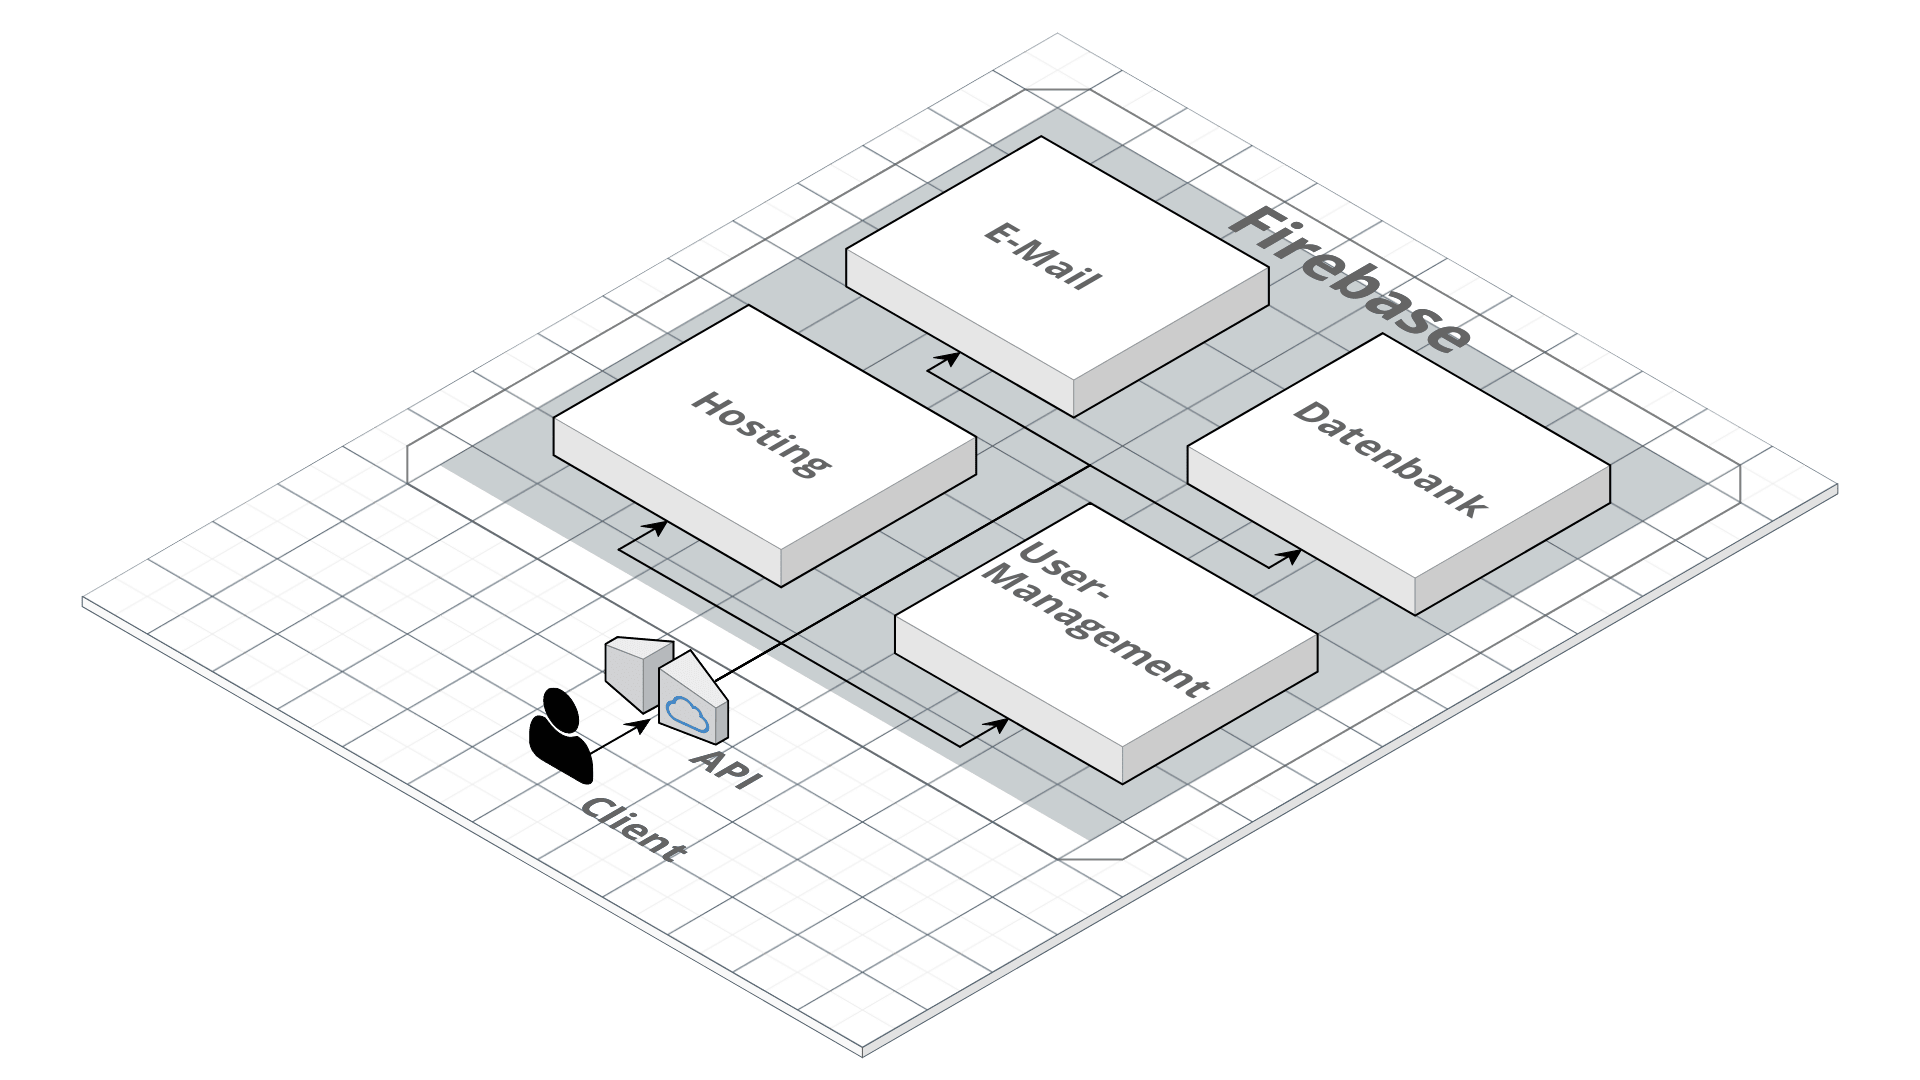
\includegraphics[width=.9\textwidth]{img/Firebase.png}
    \caption{Vereinfachter Firebase-Aufbau}
    \label{fig:firebaseAufbau}
\end{figure}


Wir haben uns für die Verwendung von Firebase als eine solche Lösung entschieden.
Firebase ist ein \ac{BaaS}-Dienst von Google LLC.
Firebase wurde aus einer Reihe von Gründen für die Entwicklung der Anwendung ausgewählt:
\begin{itemize}
    \item Datensicherheit\\
        Nach einer Befragung von Tang und Liu stimmen 48\% zu, dass Cloud-Provider eine bessere Sicherheit liefern als eigene Implementierungen.\autocite[S. 63]{TANG}
        Google als einer der größten IT-Dienstleister ist dabei weit vorne und ist konform mit den europäischen Datenschutzverordnungen.\autocite{firebaseDataprotection}
        Die Authentifizierung ist sicher, da aktuelle Standards wie OAuth 2.0 verwendet werden.
    \item Ausfallsicherheit\\
        Da Server nicht mehr einzeln betrieben werden müssen entfällt die Gefahr eines \enquote{Single Point of Failure}. 
        Dieser wäre dafür verantwortlich, dass die Anwendung ausfällt, sofern der Server abstürzen würde.
        Firebase und Google bieten stattdessen ein \ac{SLA} an, das eine Ausfallsicherheit von mehr als 99,9\% garantiert.\autocite{firebaseSLA}
    \item Komplexität\\
        Da Entwickler nun nur noch das Frontend entwickeln müssen und sich nicht mehr um das Backend oder die Kommunikation zwischen den Komponenten kümmern müssen, wird die Entwicklung vereinfacht und beschleunigt.
        Die Entwicklung des Frontends kann vorranschreiten, ohne auf die Entwicklung des Backends warten zu müssen.
    \item Kosten \\
        Google bietet attraktive Preismodelle an, welche die Bereitstellung der Anwendung sehr kostengünstig machen.
        Nicht nur entfallen Kosten für die Wartung der Server und Hardwareressourcen, sondern der gesamte Betrieb ist im \enquote{Spark}-Plan kostenlos.
    \item Skalierung \\
        Firebase kümmert sich um die gesamte Bereitstellung und Skalierung der Serverleistung.
        Das heißt, sofern mehr Rechenleistung benötigt wird (wie beispielsweise in Lastspitzen), wird die Rechenleistung automatisch erhöht und so das Fehlschlagen von Anfragen vermieden.
\end{itemize}




















\section{Konzeption der Funktionalitäten}\label{sec:konzeptionFunktionalitaeten}


\subsection{Kurse}\label{sub:konzeptionKurse}

Informationen sollen in Kurse unterteilt werden.
Aus diesem Grund wird eine Möglichkeit benötigt, wie Nutzer Kurse wechseln können und wie sie erkennen können, zu welchem Kurs die Informationen gehören.
Auch hier gibt es mehrere Möglichkeiten, wie eine solche \ac{UX} gestaltet werden kann, die jeweils verschiedenen Vor- und Nachteile besitzen.

Eine Möglichkeit ist, die gesamte Anwendung innerhalb eines Kurses anzubieten.
Das heißt, der Nutzer hat nach dem Login die Möglichkeit einen seiner Kurse auszuwählen.
Dieser Kurs wird anschließend geladen und der Nutzer sieht nur die Informationen dieses Kurses.
Möchte man den Kurs wechseln, gibt es ein Bento-Menü, über welches ein anderer Kurs ausgewählt werden kann.
Eine solche \ac{UX} hat den Vorteil, dass sich ein Nutzer vollständig auf einen Kurs konzentrieren kann und so nicht Informationen zwischen verschiedenen Kursen durcheinander wirft.
Gleichzeitig kann dies aber dazu führen, dass ein Nutzer eventuell den Überblick über seine Kurse verliert und so einen Kurs womöglich vernachlässigt.
Auch Kurs-übergreifende Informationen, z.\,B. Aufgaben, können nur schwer abgebildet werden, ohne dass die Nutzung der Anwendung erklärungsbedürftig wird.

Als zweite Möglichkeit kommt eine virtuelle Trennung zum Einsatz.
Dabei sieht der Nutzer alle Informationen und eine Trennung dieser findet nur über die Navigation statt.
So besitzt die Anwendung für jeden Kurs einen eigene Sektion, in der die Informationen dargestellt werden.
Dadurch kann der Nutzer stets alle Kurse sehen und die \ac{UX} wird vereinfacht.



\subsection{Rollenzuweisung}

Aus den Anforderungen geht hervor, dass es zwei Nutzerrollen gibt: Dozenten und Studenten.
Dozenten sollen in der Anwendung ihre Kurse verwalten können.
Ein Kurs orientiert sich dabei an der Organisation, die in der Realität vorliegt.
Auch in vorhandenen Tools wie beispielsweise \enquote{Moodle} sind Studenten anhand von Kursen organisiert.
Aufgrund der Vielzahl an solchen Lösungen scheint sich eine solche Organisation zu bewähren.
Aus diesem Grund liegt es nahe, das auch die zu entwickelnde Anwendung eine solche Struktur nutzen sollte.

Nachdem nun geklärt wurde, wie die Organisation von Studenten und Dozenten stattfindet, muss nun die Zuweisung von Studenten zu Kursen und die Zuweisung von Dozenten konzipiert werden.
Zunächst wird die Studentenzuweisung betrachtet.
Für die Zuweisung von Studenten kommen mehrere Ansätze in Betracht, die sich in der Person unterscheiden, die die Zuweisung durchführt:
\begin{enumerate}
    \item Zuweisung durch Anwendungsadministrator
    \item Zuweisung durch Dozenten
    \item Zuweisung durch Studenten
\end{enumerate}
Als erster Ansatz kommt die Zuweisung durch einen Anwendungsadministrator in Betracht.
Ein solcher Administrator ist ein zentraler Mitarbeiter der DHBW, welcher komplette Autorität über die Anwendung besitzt.
Von einem solchen Ansatz wird abgesehen, da der Verwaltungsaufwand sehr hoch wäre.
Für jeden Kurs über 20 Studenten zuzuweisen, und das für mehrere Kurse pro Semester und Vorlesung, scheint nicht realistisch.

Der zweite ist der Ansatz der Zuweisung durch einen Dozenten.
In der aktuellen DHBW-Organisation besitzen Dozenten bereits eine Liste an Studenten für ihre Vorlesung.
Diese Liste dient zur Anwesenheitskontrolle.
Demnach können Dozenten diese Liste für die Zuweisung in der Anwendung nutzen.
Der Nachteil eines solchen Ansatzes ist es aber, dass Studenten ihre Daten in der Anwendung hinterlassen müssen und diese durch andere Dozenten gegebenenfalls einsehbar wären.
Zusätzlich geht die Anonymität, welche durch Matrikelnummern gegeben ist, eventuell verloren.
Insgesamt ist dieser Ansatz aus Datenschutzaspekten besonders kritisch. 

Als letzter Ansatz ist die Zuweisung durch den Studenten denkbar.
Denkbar sind hier wieder umehrere Fälle: Eine Liste aus Kursen oder über einen Kursidentifikator.
Eine Liste mit Kursen vereinfacht die Zuweisung durch den Studenten, da Kurse schnell entdeckt werden können und eventuell zusätzliches Wissen vermittelt werden kann, wenn der Student sich für mehrere ähnliche Kurse einträgt.
Nachteil ist aber die unmittelbare Verwaltung und Übersicht über die Kurse.
Eine Zuweisung über einen Kursidentifikator (kurz: Schlüssel) hat den Nachteil, dass diese Schlüssel erst aufwändig über einen weiteren Kommunikationsweg (z.\,B. Email oder direkt in einer Vorlesung) mitgeteilt werden muss.
Dafür wüeden die  Studenten aber nur Zugriff auf die für sie relevanten Vorlesungen besitzen.
In \enquote{Moodle} ist die Zuweisung zu Kursen auf freiwilliger Basis anhand von Einschreibeschlüsseln gelöst.
Aus diesem Grund ist dieser \enquote{Workflow} bereits für Studenten bekannt und eine Anpassung an die neue Anwendung ist schnell möglich.
In der Tat nutzen viele existierende Anwendungen ein solches System.
Beispiele hierfür sind Zoom oder Google Meets.


\subsection{Registrierung}
Nutzer der Anwendung können sich selbst registrieren.
Daraus ergibt sich aber eine Rollen-Problematik: Woran kann die Anwendung erkennen, welcher Nutzer ein Student ist und welcher Nutzer ein Dozent ist?
Sofern Nutzer dies selber angeben können, bräuchte es gegebenenfalls eine Validierung durch die DHBW, wodurch erneut die oben genannten Nachteile einer Zuweisung durch einen Administrator greifen würden.
Ein Ansatz, bei dem Nutzer dies selber verwalten können wird auch hier als besser angesehen.
Aus diesem Grund wird der folgende Ansatz verwendet:
Statt festdefinierte Rollen (Student und Dozent) zu besitzen, kann jeder Student selbst sowohl Student als auch Dozent sein.

Jeder Nutzer ist zunächst keiner Rolle zugeordnet.
Jeder Nutzer kann einen Kurs erstellen, wodurch dieser Nutzer automatisch zu einem Dozent für diesen Kurs wird.
Sobald sich ein Nutzer mithilfe des Einschreibeschlüssels für einen Kurs anmeldet wird der Nutzer automatisch für diesen Kurs zu einem Studenten.
Dadurch können auch zuvor nicht vorgesehene Nutzerbeziehungen entstehen.
Beispielsweise kann ein Dozent sich in einen weiteren Kurs einschreiben, falls er sich in einer bestimmten Richtung weiterbilden möchte.
Oder die DHBW kann sich für einen Kurs einschreiben, um die Qualität einer Vorlesung zu validieren.


Ein Vorteil eines solchen Ansatzes ist es, dass auch Studenten Kurse erstellen können und so Lerngruppen gefördert werden.
Denkbar ist beispielsweise ein Student, welcher Nachhilfe anbietet.
Dadurch wird die Nutzung der Anwendung gefördert.








\subsection{Aufgaben}
Aus den Anforderungen geht hervor, dass Aufgaben gespeichert werden sollen. In Einklang mit den anderen Konzeptionen können auch die Aufgaben an Kurse gebunden werden. Stattdessen haben wir uns aber dafür entschieden, die Aufgaben zentral und Kurs-übergreifend zu gestalten. So hat der Nutzer stets Übersicht über alle Aufgaben und es geraten keine Informationen in den Hintergrund.

Neue Aufgaben sollen einfach hinzugefügt werden können. Aus diesem Grund soll es nur notwendig sein den Namen einer Aufgabe zu definieren und alle anderen Attribute wie Fälligkeitsdaten lediglich optional zu gestalten.

Gleichzeitig sollen alle Aufgaben grafisch dargestellt werden, um die Planung zu erleichtern.
Optimalerweiße sollten die Termine in einem Kalender dargestellt werden.
Je voller ein Tag ist, desto deutlicher soll der Backlog hervorgehoben werden, mit rot als Signalfarbe. Der Kalender soll prominent dargestellt werden, sodass der Nutzer sich sofort einen Überblick verschaffen kann. 


\subsection{Karteikarten}
In den Anforderungen wurde definiert, dass die Anwendung Karteikarten zur Untersützung von Lerninhalten anbieten soll.
Für das Lernen mit den Karteikarten gibt es eine Vielzahl an unterschiedlichen Algorithmen. Unsere Anwendung soll einen Algorithmus aus dem Bereich der \enquote{Spaced Repetition Systems} implementieren. In die deutsche Sprache übersetzt heißt das so viel wie "Wiederholen ohne Lücken". Das System hinter diesen Algorithmen besteht darin, die entsprechenden Informationen genau dann zu wiederholen, wenn das menschliche Gehirn sie fast schon vergessen hätte.\autocite[Vgl.][]{Tabibian3988} Die einzelnen Karteikarten werden nacheinander abgefragt und bei richtiger Antwort in zunehmenden Zeitintervallen immer wieder überprüft. Durch diesen Abstandseffekt soll gezielt das Langzeitgedächnis trainiert werden, damit die Inhalte auch über eine Prüfung hinaus im Gedächtnis behalten werden. Die unterschiedlichen Algorithmen dieser Klasse unterscheiden sich lediglich in der Wahl der Zeitabstände. 
Genutzt werden soll das Super-Memo System des polnischen Neurobiologen Piotr Wozniak. Es definiert folgende Zeitabstände:
\begin{itemize}
	\item 20 Minuten
	\item 24 Stunden
	\item 48 Stunden
	\item 10 Tagen
	\item 30 Tagen
	\item 60 Tagen
\end{itemize}  
Kann eine Frage nicht beantwortet werden, so wird diese direkt wiederholt und durchläuft die definierten Zeitintervalle von vorn. \autocite[Vgl.][]{BaileyuDavey}



\subsection{Lernmaterialien}
Um das Lernen zu unterstüzen sollen Dozenten weitere Kursinhalte in der Anwendung bereitstellen können.
Momentan müssen Dokumente umständlich an Studenten weitergegeben werden.
In der Regel werden Dokumente an die Kurssprecher geschickt, welche die Dokumente anschließend weiterverteilen.
Das Problem ist, dass zuerst die Email-Adressen der Kurssprecher ausgetauscht werden muss und diese einen zusätzlichen Aufwand haben.
So sind neue oder korrigierte Dokumente nur schwer auszutauschen.
Auch Dokumente, die während einer Vorlesung verteilt werden müssen, erzeugen eine Zeitdifferenz.
Dazu kommt, dass dieser Workflow nicht immer gleich ist.
Oft bekommen verschiedene Schüler unterschiedliche Informationen.
In einigen Fällen wird auch Moodle für die Dateiablage verwendet.
Aus diesem Grund wird ein einheitliches System benötigt, in dem Dateien abgelegt werden können.

Bei der Konzeption werden verschiedene Methoden betrachtet, mit der Dozenten Informationen an die Kursteilnehmer übergeben können.
Die einfachste Methode wäre es, Skripte per Email an die Teilnehmer zu versenden.
Hierbei würde die Anwendung wie ein Email-Verteiler wirken. Da Email-Adressen bereits für das Login benötigt werden, wären alle Informationen bereits vorhanden.
Dadurch entstünden aber neue Problematiken. Zum einen müssten weitere datenschutzrechtliche Bedenken geklärt werden, beispielsweiße die Weitergabe und Verarbeitung der Email-Adressen. Außerdem müsste sichergestellt werden, dass alle Email-Adressen gültig sind und Informationen auch zustellbar sind. Unter Umständen könnten dadurch einige Studenten Vorteile gegenüber anderen Studenten bekommen.
Dazu kommt, dass Informationen erneut unübersichtlich für Studenten wären. So kamen beispielsweiße an verschiedenen Tagen Informationen wie Skripte an, die im Posteingang durcheinander geraten würden. Womöglich würden z.\,B. Informationen von verschiedenen Vorlesungen vermischt werden, was sich negativ auf den Lernerfolg auswirken könnte.

Stattdessen wäre es besser, wenn Informationen direkt in der Anwendung einsehbar wären. Informationen können hier wie in \autoref{sub:konzeptionKurse} beschrieben durch Dozenten der einzelnen Kurse erstellt werden und stünden dann allen Kursteilnehmern zur Verfügung.\\
Auch hier stehen verschiedene Möglichkeiten zur Verfügung. Bei der Konzeption wurden verschiedene Ansätze betrachtet. Ein Beispiel hierbei ist die Überlegung, einen Text-Editor wie bei diversen Email-Providern bereitzustellen, in dem Informationen erstellt und bearbeitet werden können. Dies hat den Vorteil, dass sich die Datenhaltung vereinfacht und eine höhere Sicherheit gewährleistet würde als bei alternativen Methoden. Eine dieser alternativen Methoden ist das Hochladen von Dateien durch den Dozenten. 
Wir haben uns für letztere Methodik aus den folgenden Gründen entschieden:
Durch Datei-uploads erhöht sich zwar der Entwicklungsaufwand, der Aufwand für Nutzer wird aber stark gesenkt. So können Bilddateien und existierende Skripte einfach bereitgestellt werden, ohne dass der Dozent einen zusätzlichen Arbeitsaufwand betreiben muss.






\subsection{Dashboard}
Das Dashboard wird als Lösung für mehrere funktionale Anforderungen konzeptioniert.
Ziel des Dashboards ist es, die wichtigsten Informationen auf einen Blick zentral anzuzeigen.
Demnach sollte das Dashboard alle Informationen unabhängig von den Kursen angezeigen, sofern diese unmittelbar wichtig für den Studenten sind.
Aus den Personas, die bereits in \autoref{sec:persona} beschrieben wurden, und unserer persönlichen Erfahrung können wir einige Funktionalitäten auswählen, die wir als besonders wichtig identifizieren.
Genauer gesagt sind besonders die Klausurtermine sowie die Aufgaben, die innerhalb einer Woche anstehen, besonders wichtig.
Aus diesem Grund sollte das Dashboard genau diese Informationen in zwei Abschnitten enthalten.
Außerdem sollten keine weiteren Informationen dargestellt werden, um zu verhindern, dass das Dashboard unübersichtlich wird.

\subsection{Prüfungen}
Prüfungstermine sind essentiell, um eine gute Planung zu ermöglichen.
Aus diesem Grund wurde in den Anforderungen definiert, dass Prüfungstermine einsehbar sind.
Um zu verhindern, dass weitere Anwendungen benötigt werden und um Miskommunikationspotenzial vorzubeugen sollten alle relevanten Informationen direkt in der Anwendung editierbar sein.
Aus unserer persönlichen Erfahrung haben wir uns für die folgenden Informationen entschieden, die eintragbar sein sollten:
\begin{itemize}
    \item Name der Prüfung
    \item Beschreibung der Prüfungsleistung
    \item Datum und Uhrzeit
    \item Dauer der Prüfung
    \item Raum
    \item Zugelassene Hilfsmittel
    \item Weitere Informationen
\end{itemize} 

\subsection{Auswertungen}
Als letzte funktionale Anforderung wurde die Auswertbarkeit von statistischen Informationen definiert.
Diese sollen den Dozenten Informationen über ihre Kurse geben.
Gegenwärtig existieren Umfragen am Ende jedes Semesters, in dem Studenten die Vorlesung bewerten können.
Problematisch ist, dass diese Umfragen erst am Ende eines Semesters durchgeführt werden.
Das bedeutet, dass unter Umständen eine ganze Vorlesungsreihe suboptimal durchgeführt wird.
Dazu kommt, dass es an der DHBW einen stetigen Austausch an Dozenten gibt.
Neue Dozenten haben noch keine Erfahrung im Halten von Vorlesungen.
Viele der Dozenten bitten bereits während der ersten Vorlesungen um Feedback.
Aus diesem Grund wird eine anonyme Plattform benötigt, bei dem auch schon frühzeitiger und vor allem iterativ Feedback gegeben werden kann.

Damit ein möglichst umfängliches Stimmungsbild erhalten wird sollte ein aktiver und ein passiver Ansatz gewählt werden.
Beim aktiven Ansatz können Stundenten aktiv Feedback hinterlassen und so direkt Feedback zu Vorlesungen geben. Dadurch kann der Vorlesungsinhalt direkt mitgestaltet werden. Betrachtet werden sollen dabei die folgenden 4 Kategorien:
\begin{itemize}
    \item Spaß\\
        Ist die Vorlesung interessant gestaltet?
    \item Informationsversorgung\\
        Werden weiterführende Informationen wie Übungsaufgaben angeboten?
    \item Verständlichkeit\\
        Sind die dargestellten Vorlesungsinhalte verständlich dargestellt?
    \item Neue Informationen\\
        Wie viele Informationen vermittelt die Vorlesung?
\end{itemize}


Durch einen passiven Ansatz soll ein Dozent Einblick bekommen, welche Lernbedürfnisse Studenten des Kurses haben.
Betrachtet werden hierbei besonders, welcher Lerntyp ein Student ist, wie Affin er zu Online-Unterricht ist, die Nutzungsfrequenz von Lernapps und wie hoch die Erfahrung mit Online-Unterricht ist.
Diese Fragen sollten idealerweise vom Studenten beantwortet werden. Da diese Informationen Kurs-übergreifend sind, sollten diese bereits zu Beginnn, beispielsweise nach der Registrierung, erfragt werden.
Gleichzeitig sollte aber eine Beantwortung optional sein, damit die Fragen nicht abschreckend wirken.

Der Dozent sollte anschließend direkt innerhalb einer Anwendung eine Auswertung durchführen können, um schnell eine Übersicht zu bekommen. Gleichzeitig sollten aber alle Daten exportierbar sein. Dies würde es Nutzern ermöglichen, weitere Analysen mit anderen Hilfsmitteln durchzuführen. So können beispielsweise IBM's SQSS verwendet werden.
Aus diesem Grund sollte ein gängiges Datenformat verwählt werden. 
Besonders geeignet ist das csv Format, da es in einer Vielzahl von Anwendungen, zum Beispiel Excel, als Eingabe genutzt und weiter bearbeitet werden kann und gleichzeitig eine geringe Fehleranfälligkeit besitzt.




























\section{Datenstruktur}
Aus den in \autoref{sec:konzeptionFunktionalitaeten} entworfenen Funktionalitäten lässt sich ein Entwurf für die Datenhaltung erstellen.

Die Datenspeicherung findet vollständig innerhalb von Firebase statt.
Der hierfür genutzte Service heißt \enquote{Firestore}.
Dabei werden Daten nicht wie in einer klassischen relationalen Datenbank (\ac{RDB}) in Tabellen mit Spalten und Zeilen gespeichert, sondern in Collections aus Dokumenten. Dies erlaubt eine größere Flexibilität in der Entwicklung.


In \autoref{fig:erDiagramm} ist das zugrundeliegende Datenmodell abgebildet, welches in der Implementierung verwendet wird.

\begin{figure}[ht!] 
    \begin{center}
        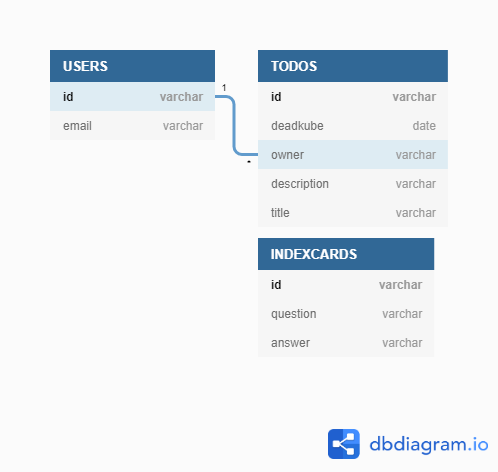
\includegraphics[width=\textwidth]{img/Integrationsseminar ER.png}
        \caption{ER-Diagramm}
        \label{fig:erDiagramm}
    \end{center}
\end{figure}





